\subsection{Parcours différencié (Julia)}
\paragraph{} Dans cette section je présenterai les parcours différenciés expérimentés auprès de mes élèves de 6\up{e} et 5\up{e}. Je porterai une attention particulière à l'évolution de ma réflexion sur ce type de dispositif suite à des lectures ou aux séances effectuées, ainsi que sur les impacts de ces réflexions sur les dispositifs que j'ai proposés. Mon analyse cherchera également à dégager l'impact de tels dispositifs pédagogiques sur l'autonomie des élèves et l'acquisition des compétences.
\paragraph{}Une de mes collègues de français pratique la classe inversée avec ma classe de 6\up{e}. Ayant lu que la classe inversée\cite{cnesco_Lafontaine}\cite{cnesco_notes_experts} pouvait être un dispositif permettant aux élèves d'acquérir une certaine autonomie tout en proposant des supports et des exercices différenciés, je me suis d'abord intéressée à ce sujet. J'ai observé mon premier parcours différencié sur le site de Mme Riguet\cite{riguet}, une enseignante qui applique la classe inversée au collège. La classe inversée m'a vite paru trop complexe à mettre en place et m'a semblé être un sujet à traiter à part entière (et non comme dispositif de différenciation). Au contraire, les parcours différenciés ont rapidement été une source d'inspiration pour moi, j'ai rapidement vu des modes de différenciations que je pouvais mettre en place et les difficultés de gestion classe qui pouvaient découler d'un mauvais calibrage du parcours.
\paragraph{}Le principe du parcours différencié est de proposer aux élèves de traiter une série d'exercices avec une progression adaptée aux difficultés que ceux-ci peuvent rencontrer. Ce parcours peut être complété par des aides progressives données par l'enseignant ou sous différents supports (capsules vidéos, document avec rappel de cours, questions intermédiaires\ldots ). \\
Dans cette section, il sera également question de parcours semi-différenciés. Les parcours semi-différenciés désignent ici des listes d'exercices à traiter par les élèves où certains exercices sont à traiter différemment selon la réussite ou non de questions précédentes (définition personnelle, je n'ai pas trouvé cette notion dans la littérature ). Un exemple d'exercice de parcours semi-différencié est présenté plus loin.
\paragraph{}
Avant de mettre en place les parcours différenciés, j'ai eu besoin de voir comment les élèves réagissaient face à une successions de travaux à faire en autonomie. J'ai donc mis en place une séance d'exercices en autonomie avec ma classe de sixième. \\
Les élèves ont commencé avec un exercice sur les fractions à faire seul, la correction et les exercices suivants se trouvant sur un ilot. J'ai ajouté une version « bis » de certains exercices disponibles pour les élèves ayant rencontré des difficultés ou voulant se rassurer. \\
Les élèves ont globalement joué le jeu, ils ont apprécié de pouvoir avancer à leur  rythme et de circuler librement dans la salle même si cela a causé de l'agitation en début de cours. Certains élèves ont cependant choisi de ne faire qu'un ou deux exercices simples, et d'autres se sont rapidement jetés sur les corrections.\\
\newline
Lors de cette expérience, je me suis rendue compte des élèves qui devaient a priori me poser des problèmes d'attitude étaient plus épanouis dans ce type de travail (lorsqu'ils faisaient l'effort d'essayer), alors que des élèves très à l'aise en condition \emph{classique} de travail individuel ont été perdus au démarrage de la première séance. De plus, une fois le dispositif en place, des élèves habituellement très discrets m'ont demandé de l'aide. J'ai cependant eu de grandes difficultés à \emph{jongler} entre les élèves. Ceux-ci étaient encore peu autonomes et avaient surtout besoin d'être rassurés. J'ai également eu du mal à estimer le temps à laisser à chacun pour travailler seul, et à identifier les moments où instaurer le travail en commun.\\
Cela m'a confortée dans l'idée que la construction de parcours différenciés, avec des étapes clés et à réaliser en autonomie par les élèves pouvait avoir un apport pédagogique intéressant pour mes classes, mais qu'il demandait un travail d'organisation en amont plus important.

\subsubsection{Premier réel parcours différencié}
J'ai décidé d'effectuer ma première expérimentation de parcours différencié avec ma classe de cinquième pour la séquence \emph{Symétrie centrale}. Nous avons commencé la séquence par un travail de rappels sur la symétrie axiale, suivie par une activité de l'IREM de Lille sur la construction par symétrie centrale\footnote{\url{https://irem.univ-lille1.fr/spip.php?article276}}.\\
J'ai construit un parcours d'exercices d'application sur la construction de symétriques pour les deux séances suivantes. J'ai distribué le parcours sans la feuille d'exercices aux élèves afin de m'assurer que les modalités ont bien été comprises. Le nouveau mode de travail a déstabilisé les élèves dans un premier temps, mais une fois face aux exercices, je n'ai eu que deux élèves perdus.\\
Pour s'aider, les élèves disposaient de l'ensemble de leurs ressources (manuels, cours, exercices déjà effectués). Ils devaient effectuer une série de six exercices autour de la construction de symétriques et disposaient d'une feuille de correction consultable à mon bureau. La liste des exercices se trouve en annexe \ref{parcours_symetrie_centrale}. Pour trois des exercices, si les élèves faisaient une erreur ou ne se sentaient pas suffisamment à l'aise, ils devaient continuer le parcours sur la branche "KO" et effectuer un exercice similaire (mêmes variables didactiques, sauf l'exercice 1 où j'ai remplacé des dessins à la main par des figures géométriques pour faciliter la compréhension).\\
Une fois les élèves en exercice, j'ai pu assister ceux qui rencontraient le plus de difficultés. J'ai remarqué qu'une majorité des élèves levait la main sans réellement chercher, ce qui parasite ce mode de travail. Je m'attendais cependant à ce phénomène, car les élèves n'étaient pas suffisamment autonomes et familiers avec l'exercice.\\
Deux élèves ont terminé la feuille d'exercice dès la première séance. Je les ai autorisés à aider des camarades en demande d'assistance dans un premier temps. Je leur ai ensuite donné des exercices de construction de symétriques supplémentaires (constructions de symétriques de figures sur feuille blanche, avec centre de symétrique hors puis dans la figure).\\
Afin de suivre leur propre progression, les élèves ont colorié leur parcours afin de retrouver leur progression à la séance suivante. Les élèves ont collé cette progression avec la feuille d'exercices sur leur cahier.\\
Le parcours a été plutôt bénéfique pour les élèves en difficulté car j'ai pu expliquer à certains leurs erreurs, d'autres ont compris par eux-même ou avec l'aide d'un camarade. Dans tous les cas, l'exercice de réinvestissement supplémentaire a été réussi (hormis pour une élève en grande difficulté et dans le refus d'écoute, à qui j'ai du redonner une feuille d'exercices).\\
Suite à la bonne conduite des séances d'exercices, et pour améliorer le travail en autonomie des élèves, je leur ai fait travailler la suite de la leçon à travers des exercices de découverte des propriétés de la symétrie centrale. Les élèves devaient travailler en autonomie, avec la possibilité d'analyser des constructions sur papier blanc et/ou sur carreaux. Encore une fois, les corrections étaient disponibles sur le bureau (dont sur papier calque pour les constructions).\\
Les élèves ont été à l'aise avec le travail en autonomie seuls 6 élèves sur 26 ont su faire le bilan de leur travail.

\paragraph{Bilan de l'expérience :}j'ai interrogé en cours de séance et de manière informelle 8 élèves généralement chahuteurs qui m'ont tous dit apprécier ce format de travail, « mais pas pour tout le temps ». 6 de ces élèves m'ont dit qu'ils s'étaient sentis perdus au départ mais qu'ils avaient pris plaisir à avancer à leur rythme, sans avoir  à attendre ou à se précipiter selon les cas. Les plus rapides m'ont dit ne pas avoir eu l'impression d'avoir travaillé lorsqu'ils réalisaient le parcours.\\
Je n'ai malheureusement pas de moyen de mesurer l'impact de l'utilisation du parcours différencié sur l'acquisition des compétences par les élèves. J'ai cependant analysé les productions de trois élèves sur le parcours différencié et lors de l'évaluation sommative. Ces analyses sont développées en annexe \ref{Prod_eleves_ju}.

\paragraph{}C'est suite à ce parcours que j'ai réalisé l'importance de poser des \textit{balises} pour la correction d'exercices ou la mise en commun du travail accompli. J'ai également eu la mauvaise surprise de comprendre à quel point les élèves ne savent pas faire le bilan de leur travail. Que cela soit de leurs propres découvertes ou des leçons travaillées en classe.\\
J'ai aussi remarqué que les élèves n'avaient pas les mêmes acquis en construction géométrique et en raisonnement, et que cela posait problème dans le déroulé du parcours différencié. En effet, des élèves à l'aise dans l'observation des situations de symétries se sont trouvés incapables de construire le symétrique d'un point car ils ne savaient pas utiliser leur règle ou leur compas correctement.\\
J'aurais pu disposer de ces informations et adapter les exercices proposés en effectuant une évaluation diagnostique en amont (sur la symétrie axiale par exemple).\\
Le parcours différencié suivant ayant été construit en parallèle de l'expérimentation de ce parcours, je n'ai pas pu effectuer de diagnostique en amont. J'ai cependant effectué une évaluation diagnostique pour une troisième expérimentation, qui sera détaillée par la suite.\\


\subsubsection{Seconde expérimentation : un parcours semi-différencié}
La seconde différenciation a été effectuée sur ma classe de sixième autour du calcul avec les nombres décimaux.\\
Les élèves ont reçu une première feuille d'exercices composée de calculs aux difficultés progressives, et suivant un parcours différencié. Dans le parcours de l'expérimentation précédente, j'ai été gênée par les termes "OK" et "KO" qui pourraient être incompris ou mal interprétés. Le premier terme peut être vu comme une validation moyenne de l'exercice, "OK j'ai vite-fait compris" alors que le second terme peut être interprété comme "J'ai été mis KO par l'exercice". J'ai donc choisi de passer par des visages souriants ou non pour indiquer l'état d'esprit suite à la résolution d'un exercice. Les élèves étant de plus hyperconnectés, je n'ai pas eu de doute quant à l'interprétation de ces \textit{smileys} (\textbf{:-)} = « tout va bien j'ai compris l'exercice, j'ai su le traiter »/  \textbf{:-()} = « Je n'ai pas su traiter l'exercice, je me suis trompé ou je n'ai pas été à l'aise pour le faire »).
\paragraph{}Pour cette série d'exercices, j'ai mis davantage de possibilités de parcours, ce qui n'a pas été facile à comprendre pour les élèves. Afin de m'assurer que tout le monde a compris comment réaliser le parcours, j'ai fait faire le premier calcul aux élèves et nous avons décidé ensemble du chemin à parcourir pour chacun en fonction du résultat trouvé. À cette étape de la séance, j'ai découvert que les élèves n'étaient pas à l'aise avec les \textit{smileys} et auraient préféré avoir des termes comme "OK"/"KO" ou "Facile"/"Oups". Les élèves se demandaient « pourquoi il y a un bonhomme triste », ce qui allait à l'encontre de l'objectif du \textit{smiley}.\\
Pour éviter les aller-retour incessants des élèves, j'ai disposé en bas de la feuille d'exercice les réponses aux calculs. Je ne les ai pas disposés les uns en dessous des autres mais en colonne afin d'éviter que les élèves ne lisent involontairement les réponses en avance.
\paragraph{}J'ai également ajouté une étape « Aide » au parcours pour les élèves faisant des erreurs à des étapes clefs. Cet ajout a été compris et bien accueilli par les élèves qui savaient quand demander de l'aide et quand essayer de comprendre par eux-même. Les élèves ayant terminé rapidement et sans erreur le premier exercice devaient me montrer leur feuille pour que je vérifie que les calculs ont bien été posés. Une fois cette vérification terminée, les plus rapides et volontaires pouvaient m'accompagner pour aider un camarade (objectif : apprendre à expliquer sans donner la réponse). Une fois qu'un tiers des élèves a terminé le parcours, les élèves pouvaient passer au second parcours.
\paragraph{} En termes de contenu, ce parcours traitait de l'addition et de la soustraction de nombres décimaux. L'objectif a été pour moi de vérifier que les élèves savent poser ce type de calcul pour ensuite résoudre des problèmes demandant de telles opérations.\\
Le parcours commence donc avec deux exercices-parcours avec des calculs graduellement plus difficiles à traiter (en les posant, même s'ils pensent savoir les faire de tête). Les élèves disposent du résultat des calculs en bas de la feuille d'exercices et peuvent me demander de l'aide après un certain nombre d'erreurs (étape « Aide »). En procédant par étape, je peux ainsi rapidement identifier les sources d'erreur des élèves dans leurs calculs et rapidement y remédier de manière individuelle.\\
\begin{figure}[!h]
	\centering
	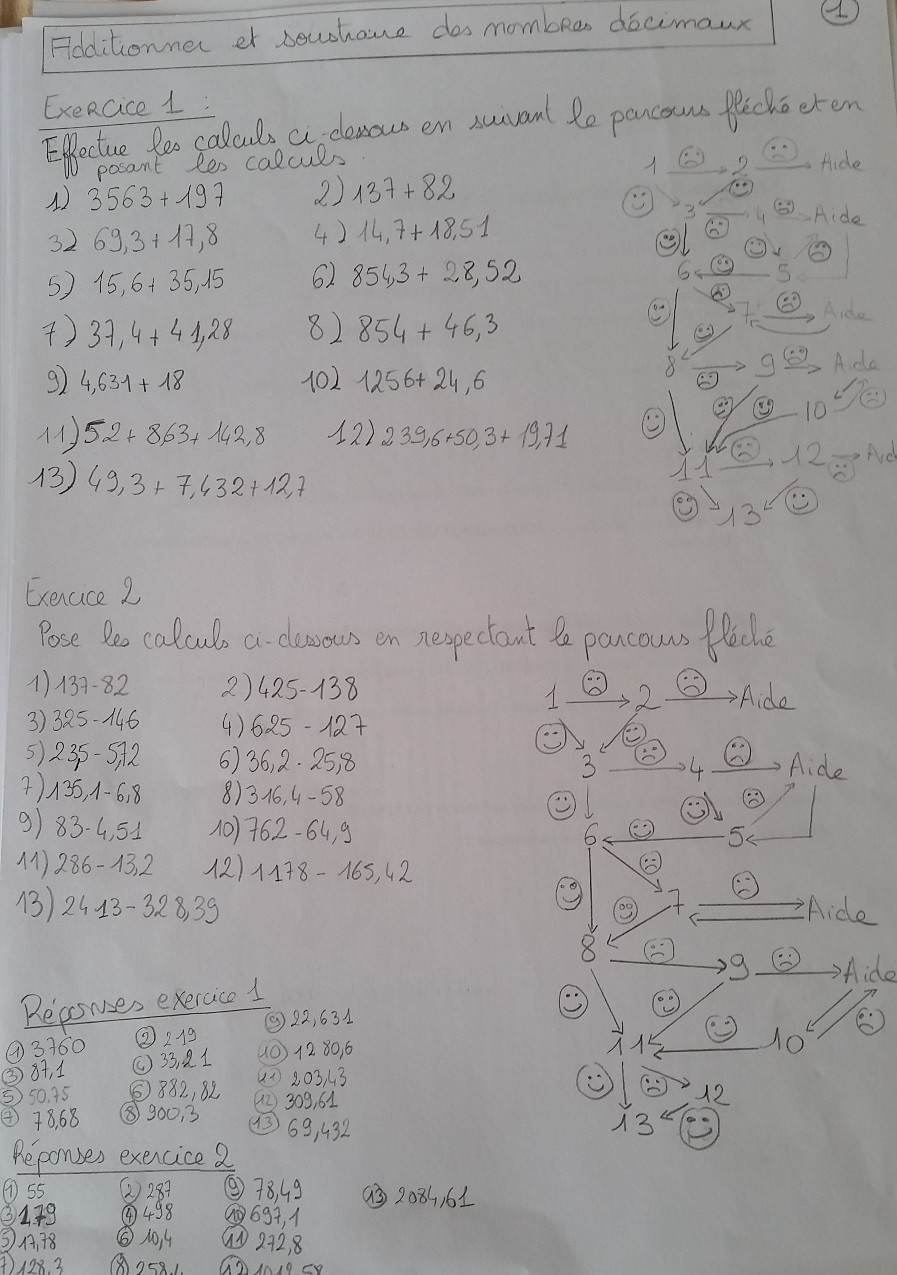
\includegraphics[scale=0.4]{img/parcours_decimaux.jpg}
	\caption{Parcours triangle}
\end{figure}
\paragraph{}Une fois les exercices traités, les élèves pouvaient passer à des problèmes graduellement plus difficiles avec la correction à disposition. Pour ces exercices, j'ai demandé aux élèves de travailler la rédaction et la présentation.

\paragraph{Bilan de l'expérimentation\\}
Dans l'ensemble, j'ai été agréablement surprise par l'esprit de travail et d'entraide qui a régné durant les séances liées à cette séquence. La séance aurait pu se dérouler de manière fluide si je n'avais cependant pas eu de problème avec des élèves très demandeurs d'attention qui refusent de travailler si on n'est pas à côté d'eux. Ces quatre élèves ont gêné l'ensemble de la classe et l'un d'entre eux a même refusé tout travail et a dû être sanctionné.\\
Le reste de la classe a terminé l'exercice et a su, avec mon aide, faire un bilan des techniques de calcul posé. J'ai remarqué moins d'erreurs de calcul par la suite lors de résolution de problèmes mais ne saurais dire si cela est dû au travail en autonomie ou au contenu même de la séquence.\\
Avec du recul, je pense que j'aurais dû rendre la prise en note du bilan obligatoire pour tous les élèves. Ceux-ci ont cependant avancé de manière hétérogène, ce qui a posé problème sur où écrire ce bilan. J'en ai retenu qu'on pouvait prévoir un espace bilan sur la feuille d'exercices, afin qu'elle soit au même endroit pour tous, et facile à retrouver. Après les parcours, les élèves devaient résoudre une série de problèmes et j'ai eu d'avantage de participation lors de la correction, avec beaucoup d'élèves demandant à exposer leur méthode de résolution.
\paragraph{}Les élèves les plus à l'aise et ne souhaitant pas aider un camarade ont cependant fini par épuiser le travail supplémentaire que j'avais prévu, ils ont donc commencé la suite de la séquence et ont même eu l'autorisation de travailler une autre matière pour l'une d'entre eux. Cela me pose la question du travail à demander à ces élèves à l'issue du parcours. J'envisage de leur demander de réaliser une carte mentale autour de la séquence et de ce qu'ils ont compris et employé lors de la séance. Nous avons d'autant plus expérimenté le jeu "Math's up" en demi-groupe\footnote{Jeu où deux équipes s'affrontent : les élèves font deviner une liste de notions mathématiques à leur équipe en les décrivant puis en dessinant lors d'une seconde manche. Pour plus d'information, voir le mémoire d'Alix Duval et d'Antonin Gelamur qui traite en détail de cette activité\cite{maths_up}}, les élèves ont apprécié l'aspect jeu et j'ai observé une amélioration du réemploi des notions par la suite en classe. Les élèves les plus avancés pourraient donc travailler sur quelles notions réemployer pour le jeu par exemple (et de partir de ces notions pour construire une carte mentale en bilan de la séance).

\subsubsection{Troisième parcours différencié (non expérimenté)}
À partir des bilans autour des deux premières séances et suite à des échanges avec Xavière, Victoire, Nadine Grapin et Marine Doceul (tutrice terrain), j'ai rapidement compris qu'il me manquait trois points importants dans mes parcours différenciés :
\begin{itemize}
	\item une évaluation diagnostique sur la notion (cycle 3) ou sur les prérequis de la séquence ;
	\item des balises claires dans le parcours et pour les élèves sur les instants où le travail doit être présenté au professeur, où il faut demander de l'aide ou lorsqu'il faut attendre une mise en commun ;
	\item un ou des moyens d'évaluer l'impact des travaux sur l'acquisition des compétences et des connaissances des élèves, dont le travail en autonomie.
\end{itemize}
\paragraph{} Pour la dernière expérimentation décrite dans le cadre du mémoire, j'ai donc choisi d'évaluer les élèves de sixième sur la séquence \textit{Quadrilatères et triangles particuliers}. L'évaluation diagnostique et son analyse se trouvent en annexe \ref{Eval_diag_ju}. J'ai profité de devoir rendre l'analyse d'une évaluation pour le portfolio pour présenter cette évaluation diagnostique.\\
Suite à cette évaluation, j'ai pu mettre en avant différents types de connaissances sur lesquelles j'ai observé des erreurs :
\begin{itemize}
	\item Connaître les propriétés du carré, rectangle ou losange (hors diagonales)
	\item Connaître les propriétés des diagonales du carré, rectangle ou losange
	\item Connaître les propriétés du triangle rectangle
	\item Connaître les propriétés du triangle isocèle ou équilatéral
	\item Comprendre la notion d'angle
	\item Comprendre la notion de diagonale
\end{itemize}
Certains élèves ont fait des erreurs sur plusieurs catégories de connaissances ; un certain nombre d'élèves n'ont pas répondu à l'évaluation. Un extrait de copies se trouve en annexe \ref{fig:Eval_diag_copies}.\\
Après analyse des difficultés de chacun, j'ai mis en place deux parcours :
\begin{itemize}
\item Quadrilatères
\item Triangles
\end{itemize}
Un exemple de parcours se trouve en annexe\ref{parcours_diff3}. Les élèves devront traiter certaines catégories d'exercices en priorité.
Les élèves à l'aise partout devront tout de même se soumettre aux exercices de chaque catégorie ne serait-ce que pour réinvestir leurs connaissances, voire aider leurs camarades (compétence \textit{travailler en groupe} du référentiel commun de compétences).\\
Une fois qu'ils ont terminé une série d'exercices, par exemple sur les triangles rectangles, si je les considère suffisamment en avance, ils pourront mettre leur nom au tableau dans la colonne \textit{Tuteur triangle rectangle}. De même, les élèves dans le besoin pourront mettre leur nom dans la colonne \textit{À aider triangle rectangle} par exemple.\\
J'ai modifié le plan de table de la classe pour rapprocher des élèves au profil « tuteur » et « demandeur d'aide » et en mettant les élèves en grande difficulté ensemble sur un îlot pour mieux les accompagner.
Les élèves seront munis de leur Ordival et auront chargé un dossier depuis un serveur avant la séance pour disposer de toutes les ressources dont ils pourraient avoir besoin (capsules vidéos, exercices GeoGebra, images \ldots).
Cette expérimentation demande un travail d'organisation important, je compte expérimenter en demi-groupe dans un premier temps, puis en classe entière.\\
J'anticipe une grande difficulté autour de la mise en commun des notions travaillées car plusieurs parcours sont effectués en même temps. Je prévois de mettre des échéances pour chaque parcours et de faire un bilan à mi-parcours et un bilan final. Mon inexpérience sur le traitement de ce chapitre en classe m'empêche de fixer plus de balises. Je profiterai cependant du temps en demi-groupe pour éventuellement traiter des points en plénière.\\
De plus, j'annoncerai en début de séance quels parcours seront priorisés pour les explications individuelles de ma part.

\subsubsection{Bilan évaluation des dispositifs}\label{retour_parcours}
 \remark{Je n'ai pas eu le temps de rédiger cette partie. Les éléments sont repris dans la partie commune}
evaluation travailler en autonomie sur pronote, 2h
questionnaire
retour évaluation
Pour les parcours différenciés, alors que les élèves les plus fragiles demandent un ajustement de certains parcours sur la forme, les élèves ont traité en moyenne deux fois plus d'exercices lors des séances en autonomie sur les séquences numériques. Les exercices de géométrie ont quant à eux été traités de manière plus difficile selon les compétences testées. De manière générale, les élèves ont traités plus d'exercices qu'à l'accoutumée, mais j'ai dû intervenir de manière plus fréquente, avec beaucoup d'interventions en plénière

